\chapter{Parsimony and Causal Inductive Bias Across Complexity Rungs}
\label{ch:parsimony_complexity}

The preceding chapter showed that synchronization, reference construction, and spectral
ambiguity all shape respiratory-rate error. This chapter asks how much additional model
complexity is justified once those measurement choices are made explicit. The experiments
progress from small changes to the quadrature front end, through causal and offline temporal
filters, to differentiable hidden-state models and unconstrained neural regressors. The central
comparison is not simply whether a more complex model can lower one RMSE. It is whether a
measured gain survives patient-level evaluation, a second reference definition, physical
perturbation tests, and constraints that prevent the model from relying on absolute-rate
shortcuts.

The primary internal cohort is \texttt{pool30\_sync}, comprising 28 sessions from 11 infants.
The frozen baseline and the Stage~1 and Stage~2 reconstructions use the same shared raw-NLS lag.
Stage~2 models are trained within patient-disjoint leave-one-patient-out (LOPO) folds using only
the monitor's one-hertz respiratory-rate channel. Their predictions are then evaluated against
that channel and against high-rate respiratory triggers. The lag-adjusted trigger evaluation,
called \texttt{Trig -10 s} in the project outputs, compensates for the monitor's observed
approximately ten-second group delay; it is a shared reference-alignment sensitivity, not a
per-model lag optimization. These results remain internal evaluations on one small cohort.
The full Stage~2 audit also retains the recorded-time trigger and the whole-window trigger-count
rate; the principal model table foregrounds the one-hertz and lag-adjusted interval-rate
references.

Figure~\ref{fig:ch4_rungs} summarizes the contrast between structured, rate-equivariant models
and higher-capacity regressors that can exploit absolute-rate correlations.
\begin{figure}[htbp]
\centering
\resizebox{\textwidth}{!}{%
\begin{tikzpicture}[
  x=1cm, y=1cm,
  font=\footnotesize\sffamily,
  >=Stealth,
  physbox/.style={
    draw=oiGreen!80!black, fill=oiSafeBg, rounded corners=3pt,
    thick, align=center, inner sep=6pt
  },
  shortcutbox/.style={
    draw=oiVermilion!85!black, fill=oiWarnBg, rounded corners=3pt,
    thick, align=center, inner sep=6pt
  },
  featbox/.style={
    draw=oiBlue!80!black, fill=oiLightBg, rounded corners=3pt,
    thick, align=center, inner sep=6pt
  },
  statpill/.style={
    draw=oiGray!65, fill=white, rounded corners=2pt,
    thin, align=center, inner sep=5pt, font=\scriptsize\sffamily
  }
]

% Left Input Node centered vertically at y = 3.35
\node[featbox, text width=3.65cm, minimum height=6.40cm] (input) at (1.90, 3.35)
  {\textbf{Folded Harmonic}\\ \textbf{Salience Tensor}\\$\mathbf{\Phi}_t \in \mathbb{R}^{K_q \times d}$\\[7pt]
   $6$ orthogonal channels\\across grid $q\in[18,90]$\,bpm:\\[5pt]
   \scriptsize $P_{\mathrm{clean}}(f),\; P_{\mathrm{clean}}(2f)$\\[2pt]
   $P_{\mathrm{clean}}(3f),\; P_{\mathrm{clean}}(f/2)$\\[2pt]
   $\phi_{\mathrm{anchor}},\; P_{\mathrm{raw}}(f)$\\[8pt]
   \scriptsize $SO(2)\times\mathbb{R}_{>0}$-invariant,\\zero-leakage \texttt{csd()} + HPSS};

% Top Branch: Rung 1 & Rung 2 Equivariant Path (y = 5.45 -> ~0.95 cm clear above bottom box)
\node[physbox, text width=6.35cm, minimum height=2.25cm] (r2) at (7.80, 5.45)
  {\textbf{Rung 1 (3p) \& Rung 2 FilterSafe-8 (8p):}\\
   \textbf{Shift-Equivariant Differentiable 1D-HMM}\\[5pt]
   $\eta_t(q) = \sum_m w_m \Phi_{t,m}(q)$ (zero absolute bin weights)\\
   Exact BPTT Forward--Backward ($\le\num{3.6e-9}$ grad err)\\
   Shift equivariant: $+10\,\mathrm{bpm}$ err $= \SI{1.4e-14}{\bpm}$};

\node[statpill, text width=4.20cm, minimum height=2.25cm, right=0.55cm of r2] (r2res)
  {\textbf{Dual-Reference \& \texttt{L4} Verified}\\[3pt]
   NICU 1\,Hz: $\mathbf{6.849}$ ($p_{\mathrm{Holm}}=\mathbf{0.0117}$)\\
   NICU Trig $-10\,\mathrm{s}$: $\mathbf{8.063}$ ($p_{\mathrm{Holm}}=\mathbf{0.0215}$)\\
   \texttt{gleichauf2024}: $\mathbf{0.0197}$\,bpm, slope $\mathbf{0.9994}$\\
   20\,bpm skirt: $\mathbf{0.0949}$\,bpm\\
   80\,bpm in-band: $\mathbf{0.0089}$\,bpm};

% Bottom Branch: Rung 3 Shortcut Path (y = 1.25)
\node[shortcutbox, text width=6.35cm, minimum height=2.25cm] (r3) at (7.80, 1.25)
  {\textbf{Rung 3 (439--15,817p):}\\
   \textbf{Unconstrained Absolute-Frequency Regressors}\\[5pt]
   \texttt{R3c} Ridge (439p), \texttt{R3b} MLP (15k), \texttt{R3a} TCN (16k)\\
   Break translation symmetry $\implies$ memorize VitaGuard\\
   \SI{10}{\second} trend lag \& training cohort prior ($\sim\SIrange{45}{50}{\bpm}$)};

\node[statpill, text width=4.20cm, minimum height=2.25cm, right=0.55cm of r3] (r3res)
  {\textbf{In-Band Illusion / \texttt{L4} Collapse}\\[3pt]
   NICU 1\,Hz: $5.798$--$6.584$\,bpm (variance $\times 0.52$)\\
   NICU Trig $-10\,\mathrm{s}$: $8.102$--$8.515$ ($p_{\mathrm{Holm}}=1.00$)\\
   \texttt{gleichauf2024}: $\mathbf{3.18}$--$\mathbf{3.64}$\,bpm (slope $0.709$)\\
   20\,bpm skirt: $\mathbf{11.78}$--$\mathbf{32.70}$\,bpm collapse};

% Connections
\draw[->, very thick, oiGreen!80!black] (input.east) |- (r2.west);
\draw[->, very thick, oiGreen!80!black] (r2.east) -- (r2res.west);
\draw[->, very thick, oiVermilion!85!black] (input.east) |- (r3.west);
\draw[->, very thick, oiVermilion!85!black] (r3.east) -- (r3res.west);

\end{tikzpicture}%
}
\caption[Physical Equivariance vs.\ Shortcut Complexity Architecture]{Architectural contrast across the Stage~2 Complexity Ladder (\texttt{Rung 1--3}): weight-shared zero-offset 1D-HMM operators (\texttt{R1a}, \texttt{R2e FilterSafe-8}) preserve exact translation equivariance and transfer zero-touch to \texttt{gleichauf2024}, whereas unconstrained absolute-frequency regressors (\texttt{R3c}, \texttt{R3b}, \texttt{R3a}) memorize VitaGuard \SI{1}{\hertz} smoothing and the NICU rate prior.}
\label{fig:ch4_rungs}
\end{figure}


\section{Two references and the measurement-time problem}
\label{sec:ch4_references}

The Stage~1 benchmark carries forward the distinction between the one-hertz
\texttt{RespRate} monitor stream and the high-rate respiratory trigger series. In the primary
cohort, the trigger-derived interval rate differs from the monitor rate by a mean of
$+2.15$~bpm when pooled across windows and $+1.65$~bpm when averaged equally across sessions,
with differences defined as trigger rate minus monitor rate.
Its window-level mean absolute difference is $5.03$~bpm (Table~\ref{tab:ch4_dual_reference}), and its within-session association with
the monitor is $\rWithin=0.606$ at zero offset. These are comparisons between two measurement
constructions, not an adjudication that either one is a universal ground truth.

The trigger interval rate is computed from inter-trigger gaps after excluding gaps longer than
five seconds. Consequently, windows containing pauses can report the rate of the breaths that
occurred while omitting the time spent without a breath. A whole-window count rate,
\texttt{br\_trig\_count\_bpm}, makes the opposite choice and includes the pauses in its
denominator. Relative to the one-hertz rate, the count-based estimate has a pooled difference of
$-7.08$~bpm overall and $-13.52$~bpm in windows containing a greater-than-five-second gap.
These pause-like intervals are not clinically adjudicated apnea events. The contrast shows that
the target rate depends on the reference definition, especially during quiet intervals.

\begin{table}[htbp]
  \centering
  \footnotesize
  \setlength{\tabcolsep}{4.5pt}
  \caption{One-hertz monitor and respiratory-trigger comparison under the shared Stage~1
  alignment. Differences are trigger rate minus monitor rate; the trigger interval estimator
  excludes inter-trigger gaps longer than five seconds.}
  \label{tab:ch4_dual_reference}
  \begin{tabularx}{\textwidth}{@{}>{\raggedright\arraybackslash}Xrrrrr@{}}
    \toprule
    Cohort & Sessions & Monitor win & Trigger win & Mean diff (sess / pool) & MAE (pool) \\
    \midrule
    \texttt{pool30\_sync} & 28 & 6,640 & 6,638 & $+1.65 / +2.15$ & 5.03 \\
    \texttt{retained23} & 23 & 6,447 & 6,445 & $+1.64 / +2.13$ & 5.01 \\
    \texttt{PAPER\_18} & 18 & 5,466 & 5,466 & $+1.39 / +1.69$ & 4.65 \\
    \texttt{all\_paired} & 31 & 7,103 & 7,101 & $+1.69 / +2.21$ & 5.18 \\
    \bottomrule
  \end{tabularx}
\end{table}

The two rate streams also differ in time. Across the 28 primary-cohort sessions, their
within-session correlation rises from $0.606$ at zero lag to $0.706$ at the audited ten-second
offset between the streams. This pattern is consistent with an
effective monitor group delay in these recordings. It is not an independent measurement of a
hardware specification. The causal forward estimate in Stage~1 adds its own delay: R1a's peak
association occurs at $+6$~s against the one-hertz stream and $+16$~s against the trigger stream.
The offline R1f smoother peaks at $+4$~s and $+14$~s, respectively. Results against the trigger
at zero offset therefore mix rate-estimation error with both monitor and estimator timing.

For that reason, the experiments report both the trigger at its recorded timing and the shared
\texttt{Trig -10 s} evaluation. The latter helps separate the common monitor delay from differences
between models. Neither alignment can remove the reference's pause definition or turn these
monitor-derived measurements into clinically adjudicated labels.

\section{Stage 1 front-end parsimony}
\label{sec:ch4_frontend_parsimony}

\subsection{WP1: I/Q preprocessing gate}
\label{sec:ch4_wp1}

The locked front end starts with mean-centered complex demodulation of the I/Q samples and the
frozen signal-processing chain. WP1 tested whether clipping repair or symmetric whitening could
improve that reference without adding avoidable axis dependence. The six alternatives were
channel-wise or joint interpolation at ADC rail hits, three symmetric whitening strengths, and a
combined clipping-and-whitening treatment. All were evaluated against both the monitor and the
high-rate trigger reference.

None of the six alternatives has patient-level Holm-adjusted support on either reference
(Table~\ref{tab:ch4_wp1}): all adjusted $p$-values are $1.000$. The largest point improvement
among the whitening variants on the one-hertz reference is small relative to between-session
variation and is not reproduced as a supported result on the trigger reference. The sentinel
sessions reinforce the concern. For example, the heavily clipped sentinel Session~2.3
(18.5\% ADC rail clipping) moves from 11.73~bpm under the locked method to 13.95--14.31~bpm
for standalone whitening (13.71~bpm under combined clipping-and-whitening \texttt{F3});
Session~11.1 moves from 12.65~bpm to 12.78--13.21~bpm for standalone whitening (12.98~bpm under
\texttt{F3}). In addition, channel-wise interpolation and the combined channel-wise
procedure depend on the I/Q axes and do not preserve the same unconditional rotation invariance
as the locked complex representation.

\begin{table}[htbp]
  \centering
  \footnotesize
  \setlength{\tabcolsep}{4pt}
  \caption{WP1 front-end ablation on \texttt{pool30\_sync}. Every candidate's patient-level
  Holm-adjusted comparison with the locked anchor is non-significant on both references.}
  \label{tab:ch4_wp1}
  \begin{tabularx}{\textwidth}{@{}>{\raggedright\arraybackslash}p{4.1cm}rrr>{\raggedright\arraybackslash}p{2.2cm}>{\raggedright\arraybackslash}X@{}}
    \toprule
    Method & $\rmseSess$ (1\,Hz) & $\Delta_{1\mathrm{Hz}}$ & $\rmseSess$ (Trig) & $p_{\mathrm{pat,Holm}}$ (1\,Hz / Trig) & Note \\
    \midrule
    F0 locked CSD & 7.817 & anchor & 8.968 & -- & Locked reference \\
    F1a channel clip repair & 7.832 & $+0.014$ & 8.963 & 1.000 / 1.000 & Axis-dependent mask \\
    F1b joint clip repair & 7.831 & $+0.014$ & 8.966 & 1.000 / 1.000 & Conditional shared mask \\
    F2a sym.\ whitening ($\lambda_{\mathrm{wh}}=0.05$) & 7.804 & $-0.014$ & 8.949 & 1.000 / 1.000 & No supported gain \\
    F2b sym.\ whitening ($\lambda_{\mathrm{wh}}=0.10$) & 7.833 & $+0.015$ & 8.976 & 1.000 / 1.000 & No supported gain \\
    F2c sym.\ whitening ($\lambda_{\mathrm{wh}}=0.25$) & 7.689 & $-0.128$ & 8.804 & 1.000 / 1.000 & Sentinel degradation \\
    F3 clipping + whitening & 7.812 & $-0.006$ & 8.935 & 1.000 / 1.000 & Axis-dependent clipping \\
    \bottomrule
  \end{tabularx}
\end{table}

The Gate~G1 decision is therefore \texttt{RETAIN\_F0\_CSD\_LOCKED}. This is a parsimony
decision under the registered statistical and symmetry criteria, not a claim that the current
front end is optimal for every receiver fault. A preprocessing step should be retained only when
it delivers a reproducible benefit without introducing a new failure mode.

\subsection{WP2: the HPSS lookahead--equivalence trade-off}
\label{sec:ch4_wp2}

WP2 varied the short-time Fourier transform (STFT) window, frequency restriction, and amount of
future context used by harmonic--percussive source separation (HPSS). The locked reference,
\texttt{H0}, uses the rectangular $48/16/256$ STFT configuration and the existing 64-tap
zero-phase Kaiser FIR bandpass over $[0.30,3.00]$~Hz with $\kaiserBeta=6.5$. The bandpass is the
project's locked filter throughout Stages~0--4; it is not a Butterworth alternative. The HPSS
windowing variants range from three seconds of STFT lookahead to zero seconds
(Table~\ref{tab:ch4_wp2}).

\begin{table}[htbp]
  \centering
  \footnotesize
  \setlength{\tabcolsep}{4.5pt}
  \caption{WP2 HPSS window and lookahead ablation. Runtime is HPSS milliseconds per window;
  the error columns use the monitor and the recorded-time respiratory trigger.}
  \label{tab:ch4_wp2}
  \begin{tabularx}{\textwidth}{@{}>{\raggedright\arraybackslash}Xrrrrr@{}}
    \toprule
    Method & STFT lookahead & ms/win & Speedup & $\rmseSess$ (1\,Hz) & $\rmseSess$ (Trig 0\,s) \\
    \midrule
    H0 locked rectangular, full band & 3\,s & 3.47 & 1.00$\times$ & 7.817 & 8.968 \\
    H1 Hann COLA, full band & 3\,s & 3.69 & 0.94$\times$ & 7.999 & 9.113 \\
    H2 Hann COLA, in band & 3\,s & 2.38 & 1.46$\times$ & 8.068 & 9.146 \\
    H3 causal Hann COLA, 2-hop context & 2\,s & 2.37 & 1.46$\times$ & 8.121 & 9.074 \\
    H4 causal Hann COLA, 1-hop context & 1\,s & 2.35 & 1.47$\times$ & 8.176 & 9.235 \\
    H5 causal Hann COLA, no STFT lookahead & 0\,s & 2.35 & 1.47$\times$ & 8.267 & 9.398 \\
    H6 causal rectangular, no STFT lookahead & 0\,s & 3.41 & 1.02$\times$ & 8.079 & 9.303 \\
    \bottomrule
  \end{tabularx}
\end{table}

The faster in-band variants trade some accuracy for runtime. More importantly, the zero-STFT-
lookahead candidates do not meet the prespecified $\pm0.50$~bpm equivalence criterion against
\texttt{H0} on both references and at both session and patient levels. For \texttt{H5}, the
session/patient TOST $p$-values are $0.414/0.519$ on the one-hertz reference and $0.412/0.431$
on the trigger reference. For \texttt{H6}, the corresponding values are $0.053/0.027$ and
$0.231/0.186$; equivalence fails at least one required level. The point estimate for \texttt{H5}
is only 0.449~bpm worse than the locked anchor, but a point estimate inside the margin is not
enough to establish equivalence.

Gate~G2 therefore retains \texttt{H0\_Locked\_Rect\_Full\_L3} as the primary front end and carries
\texttt{H5} as a zero-STFT-lookahead ablation. This result sets an important boundary for
subsequent use of the word causal: the Rung~1 and Rung~2 state decoders can use no future
sequence windows while still receiving features from an HPSS front end with three seconds of
STFT lookahead. For \texttt{H5}, zero lookahead refers only to HPSS/STFT frame context. The
evaluated path also uses block-level envelope normalization and a zero-phase outer bandpass, so
it does not establish a fully frame-causal, zero-latency pipeline. It does not pass the
equivalence gate.

\section{Rung 1: temporal structure and the causality frontier}
\label{sec:ch4_rung1}

Rung~1 adds a small temporal model to the locked HPSS-NLS estimates. Its three-parameter
forward-MMSE form updates a breathing-rate posterior over the $[18,90]$~bpm candidate grid using the current
window's evidence and a transition model. At each step it reports the posterior mean without
backtracking through future windows. The MAP variant reports the most probable state, while the
fixed-lag and offline variants deliberately use increasing amounts of future context. The
comparison in Table~\ref{tab:ch4_rung1} tests both whether temporal continuity is useful and how
much latency is required to obtain it.

\begin{table}[htbp]
  \centering
  \footnotesize
  \setlength{\tabcolsep}{4pt}
  \caption{Rung~1 causality frontier on \texttt{pool30\_sync}. Block lookahead describes sequence
  decoding; STFT lookahead describes HPSS frame context, not total pipeline latency. The H0-backed
  rows retain three seconds of STFT lookahead; $\accTau{10}$ reports the equal-session mean of
  per-session strict $|e_{s,w}|<10$~bpm accuracy on the one-hertz reference.}
  \label{tab:ch4_rung1}
  \begin{tabularx}{\textwidth}{@{}>{\raggedright\arraybackslash}Xrrrrrr@{}}
    \toprule
    Method & Params & Blk / STFT & $\rmseSess$ (1\,Hz) & $\accTau{10}$ (1\,Hz) & $\rWithin$ (1\,Hz) & $\rmseSess$ (Trig 0\,s) \\
    \midrule
    R0 locked HPSS-NLS & 0 & 0 / 3\,s & 7.817 & 79.4\% & 0.423 & 8.968 \\
    R1a forward MMSE & 3 & 0 / 3\,s & 6.990 & 82.6\% & 0.454 & 8.624 \\
    R1b forward MAP & 3 & 0 / 3\,s & 7.458 & 80.0\% & 0.389 & 8.987 \\
    R1c fixed-lag MMSE & 3 & 4 / 3\,s & 6.893 & 83.0\% & 0.473 & 8.402 \\
    R1d fixed-lag MMSE & 3 & 8 / 3\,s & 6.787 & 83.4\% & 0.479 & 8.246 \\
    R1e fixed-lag MMSE & 3 & 16 / 3\,s & 6.759 & 83.8\% & 0.484 & 8.083 \\
    R1f offline FB MMSE & 3 & $\infty$ / 3\,s & 6.395 & 86.2\% & 0.454 & 7.789 \\
    R1g offline Viterbi & 2 & $\infty$ / 3\,s & 6.498 & 85.2\% & 0.439 & 7.876 \\
    R1h H5 zero-STFT MMSE & 3 & 0 / 0\,s & 7.136 & 82.6\% & 0.396 & 8.864 \\
    R1i H6 zero-STFT MMSE & 3 & 0 / 0\,s & 7.119 & 82.6\% & 0.392 & 8.917 \\
    \bottomrule
  \end{tabularx}
\end{table}

The forward-MMSE estimate improves equal-session RMSE from 7.817 to 6.990~bpm against the
one-hertz reference, with $\rWithin=0.454$. Its recorded-time trigger RMSE is 8.624~bpm. Allowing
fixed lag improves the point estimates further, reaching 6.759~bpm at 16~s, while full
forward--backward smoothing reaches 6.395~bpm. These offline results are useful upper-context
comparators, not online alternatives: they use future windows and cannot be emitted at the time
of measurement. The forward filter's improvement over R0 is also not a clinical performance
claim; the trigger timing and pause definition still affect the measured error.

The R1a--R1g paired audit illustrates the uncertainty at this cohort size. R1a's RMSE is
0.493~bpm higher than offline Viterbi under the one-hertz reference; its patient-level Holm
adjusted $p$-value is $0.0957$. Against the recorded-time trigger, the difference is
$+0.748$~bpm and the adjusted patient-level $p$-value is $0.0078$. The offline advantage is
therefore clearer on the physical trigger at zero offset, where filter and monitor delays both
affect agreement. It should not be interpreted as an equal-latency comparison.

Two controls test whether the forward filter is merely producing a smooth, inertial trace. First,
the shifted-grid midpoint audit compares candidate ranges $[18,90]$ and $[18,120]$~bpm on five
sessions. The legacy wide-transition, high-floor filter (8~bpm transition width and 0.05 uniform floor) changes its bias by $+0.26$~bpm, and a memoryless naive
MMSE estimator changes by $+2.82$~bpm. The equivariant forward-MMSE and forward--backward
operators show $+0.00$~bpm shift. Second, in five radar phase-scramble runs, the R1a
within-session correlation falls from $0.454$ to $0.006$ and its RMSE rises from 6.990 to
8.513~bpm. The scrambled input retains Fourier magnitude while losing the original temporal
phase structure. These checks support the intended response to signal structure; they do not
prove that all real-world failures are represented by the surrogate.

\section{Rungs 2 and 3: structured learning versus shortcut capacity}
\label{sec:ch4_complexity}

Stage~2 compares a compact differentiable hidden Markov model (HMM) with substantially larger
regressors. The HMM assigns each candidate respiratory rate a shared emission score derived from
six salience channels: clean-signal power at the fundamental and harmonics, a subharmonic cue, a
coarse autocorrelation anchor, and raw-signal fundamental power. Rung~2 then combines those
scores with a symmetric transition matrix built from a mixture of slow and jump components.
The transition model contains no global uniform component, and the emission weights do not
depend on the absolute rate bin. This structure makes the operator translation-equivariant over
the tested interior grid and discourages a learned preference for one absolute breathing rate.
Differentiable sequence models and their use in structured prediction provide methodological
precedent for this design \citep{mensch2018differentiable,riou2023pesto}.

The primary Rung~2 model, \texttt{R2e}, has eight learned parameters. It uses only three
passband-safe channels---clean fundamental power, the autocorrelation anchor, and raw
fundamental power---along with two symmetric smoothing taps and three transition parameters.
Restricting the evidence to these channels avoids relying on harmonic bins that cross the
locked $0.30$--$3.00$~Hz filter boundaries as the candidate rate changes. \texttt{R2a} uses all
six channels with eleven parameters; \texttt{R2b} uses a 43-parameter nonlinear residual model.
The offline Rung~2 models use the same emissions with future-window smoothing.

Rung~3 consists of a 439-parameter ridge regressor, a 14,593-parameter spectral multilayer
perceptron, and a 15,817-parameter causal temporal convolutional network. These models can fit
more flexible mappings from the training salience to rate, but they have no explicit
rate-translation equivariance constraint. They are therefore informative shortcut-learning
foils: a low in-distribution error may reflect monitor smoothing, the training cohort's rate
distribution, or other stable correlations rather than a representation that transfers when the
rate itself changes \citep{geirhos2020shortcut}.

All models are trained within patient-disjoint LOPO folds using only \texttt{br\_1hz\_30s}. The
one-hertz results are therefore the training-reference evaluation; the recorded-time and
lag-adjusted trigger results are blind reference evaluations. Table~\ref{tab:ch4_complexity_ladder} reports equal-session and
window-pooled RMSE for both references, within-session association, and the equal-session mean
of the per-session prediction-to-reference standard-deviation ratio. A ratio below one means
that, on average across sessions, the predictions vary less than the reference; it can
accompany a favorable average error when the estimator compresses the dynamic range.

\begin{table}[htbp]
  \centering
  \scriptsize
  \setlength{\tabcolsep}{3.5pt}
  \caption{Stage~2 complexity ladder on \texttt{pool30\_sync}. Lookahead is block-decoder
  lookahead / HPSS STFT frame lookahead in seconds; the latter is not total pipeline latency.
  The SD-ratio column gives equal-session mean prediction-to-reference standard-deviation
  ratios for 1\,Hz and lag-adjusted trigger (\texttt{T10}).}
  \label{tab:ch4_complexity_ladder}
  \begin{tabularx}{\textwidth}{@{}>{\raggedright\arraybackslash}Xrcc rrr c rrr@{}}
    \toprule
    & & & \multicolumn{3}{c}{\textbf{1\,Hz Monitor Reference}} & & \multicolumn{3}{c}{\textbf{Trig $-10$\,s Reference}} \\
    \cmidrule(lr){4-6} \cmidrule(l){8-10}
    Model & Params & Blk/STFT & $\rmseSess$ & $\rmsePool$ & $\rWithin$ & SD (1\,Hz / T10) & $\rmseSess$ & $\rmsePool$ & $\rWithin$ \\
    \midrule
    R0 locked & 0 & 0 / 3 & 7.817 & 7.970 & 0.423 & 1.66 / 0.99 & 8.727 & 8.579 & 0.402 \\
    R1a forward MMSE & 3 & 0 / 3 & 6.990 & 7.337 & 0.454 & 1.36 / 0.82 & 8.197 & 8.299 & 0.408 \\
    R1f offline FB & 3 & $\infty$ / 3 & 6.395 & 6.745 & 0.454 & 1.16 / 0.70 & 7.597 & 7.722 & 0.430 \\
    R1g offline Viterbi & 2 & $\infty$ / 3 & 6.498 & 6.913 & 0.439 & 1.20 / 0.73 & 7.715 & 7.924 & 0.408 \\
    R2e causal FilterSafe-8 & 8 & 0 / 3 & 6.849 & 7.186 & 0.465 & 1.36 / 0.82 & 8.063 & 7.969 & 0.441 \\
    R2a causal linear & 11 & 0 / 3 & 6.870 & 7.340 & 0.496 & 1.40 / 0.84 & 8.350 & 8.672 & 0.455 \\
    R2b causal MLP & 43 & 0 / 3 & 6.991 & 7.423 & 0.477 & 1.36 / 0.82 & 8.502 & 8.829 & 0.424 \\
    R2f offline FilterSafe-8 & 8 & $\infty$ / 3 & 6.847 & 7.184 & 0.462 & 1.29 / 0.79 & 7.879 & 7.944 & 0.436 \\
    R2c offline linear & 11 & $\infty$ / 3 & 6.941 & 7.225 & 0.444 & 1.32 / 0.79 & 8.197 & 8.210 & 0.427 \\
    R2d H5 zero-STFT HMM & 11 & 0 / 0 & 7.115 & 7.320 & 0.437 & 1.50 / 0.87 & 8.578 & 8.364 & 0.409 \\
    R3c spectral ridge & 439 & 0 / 3 & 5.798 & 6.785 & 0.490 & 0.88 / 0.55 & 8.102 & 8.724 & 0.425 \\
    R3b spectral MLP & 14,593 & 0 / 3 & 6.584 & 6.863 & 0.481 & 1.35 / 0.82 & 8.515 & 8.652 & 0.412 \\
    R3a causal TCN & 15,817 & 0 / 3 & 6.075 & 6.906 & 0.466 & 0.84 / 0.52 & 8.498 & 8.829 & 0.404 \\
    \bottomrule
  \end{tabularx}
\end{table}

The unadjusted one-hertz ranking favors the more flexible Rung~3 models: R3c reaches
5.798~bpm and R3a 6.075~bpm, compared with 6.849~bpm for R2e. That ordering changes against
the lag-adjusted physical trigger. R2e reaches 8.063~bpm, R3c 8.102~bpm, R3a 8.498~bpm, and
R3b 8.515~bpm. Relative to the one-hertz results, the R3c and R3a predictions also retain only
$0.55$ and $0.52$ of the trigger-reference standard deviation. The combination of an attractive
training-reference RMSE, reduced prediction spread, and a weaker result under the second
reference is consistent with shortcut dependence; the table alone does not prove the causal
mechanism for any individual model.

The capacity comparison also reflects differences in the fitting protocol. For the LOPO scores in
Table~\ref{tab:ch4_complexity_ladder}, every outer fold excludes its test infant. R3a and R3b use
one additional, fold-specific inner-validation infant for model selection, leaving nine infants
for network fitting; the validation infant rotates across folds. R3c and the R2 models use all ten
outer-training infants. Separately, the full-cohort foils frozen for Stage~4 use Patient~12 as the
R3a/R3b validation infant, leaving ten infants for fitting, while R3c and R2 use all eleven. Those
full-cohort refits do not generate the LOPO scores in the table. The Rung~3 results are useful as
shortcut stress tests, but neither comparison isolates parameter count from training-data access.

\begin{table}[htbp]
  \centering
  \small
  \caption{Patient-level paired comparisons for the eight-parameter R2e model. Negative
  differences favor R2e. Holm adjustment is applied within the prespecified comparison family.}
  \label{tab:ch4_r2e_inference}
  \begin{tabularx}{\textwidth}{@{}lXrrr@{}}
    \toprule
    Contrast & Reference & Mean difference [95\% CI] (bpm) & Patient wins & $p_{\mathrm{pat,Holm}}$ \\
    \midrule
    R2e vs.\ R0 & 1~Hz monitor & $-0.969\;[-1.135,-0.803]$ & 11/11 & 0.0117 \\
    R2e vs.\ R0 & Trig $-10$~s & $-0.663\;[-0.883,-0.446]$ & 10/11 & 0.0215 \\
    R2e vs.\ R1a & 1~Hz monitor & $-0.142\;[-0.335,+0.035]$ & 9/11 & 0.6641 \\
    R2e vs.\ R1a & Trig $-10$~s & $-0.134\;[-0.497,+0.166]$ & 7/11 & 1.0000 \\
    \bottomrule
  \end{tabularx}
\end{table}

R2e is the only causal architecture in this comparison that passes patient-level Holm correction
against R0 on both the one-hertz and lag-adjusted trigger references
(Table~\ref{tab:ch4_r2e_inference}). Its mean paired differences
are $-0.969$~bpm and $-0.663$~bpm, respectively. This supports R2e over the zero-parameter
baseline within the stated evaluation. It does not show that eight parameters outperform the
three-parameter R1a forward filter: R2e's patient-level adjusted $p$-values against R1a are
$0.6641$ and $1.0000$. On the one-hertz reference, the prespecified $\pm0.50$~bpm TOST supports
equivalence between R2e and R1a at session and patient levels; the corresponding patient-level
equivalence test does not pass for the lag-adjusted trigger. The defensible conclusion is that
the compact structured model improves on R0 across the two references, while the local data do
not establish a reliable gain over the simpler causal R1a filter.

The patient-level Holm-adjusted comparisons of the Rung~3 foils with R0 sharpen this distinction.
On the one-hertz reference, the adjusted $p$-values are $0.0342$ for R3a, $0.0586$ for R3c, and
$0.1289$ for R3b. On the lag-adjusted trigger, all three are $1.0000$; their patient win counts
are 8/11, 8/11, and 6/11, respectively. Thus R3a's one-hertz result does not reproduce as
patient-level evidence against R0 under the second reference.

On the recorded-time trigger, R2e's $\rmseSess$ is 8.473~bpm, compared with 8.968~bpm for R0,
8.624~bpm for R1a, and 8.255~bpm for R3c. These zero-offset comparisons are affected by the
observed monitor delay and the causal filter's group delay. The adjusted trigger comparisons are
therefore reported alongside them rather than substituted for them
(Figure~\ref{fig:ch4_complexity_ladder}).

\begin{figure}[htbp]
  \centering
  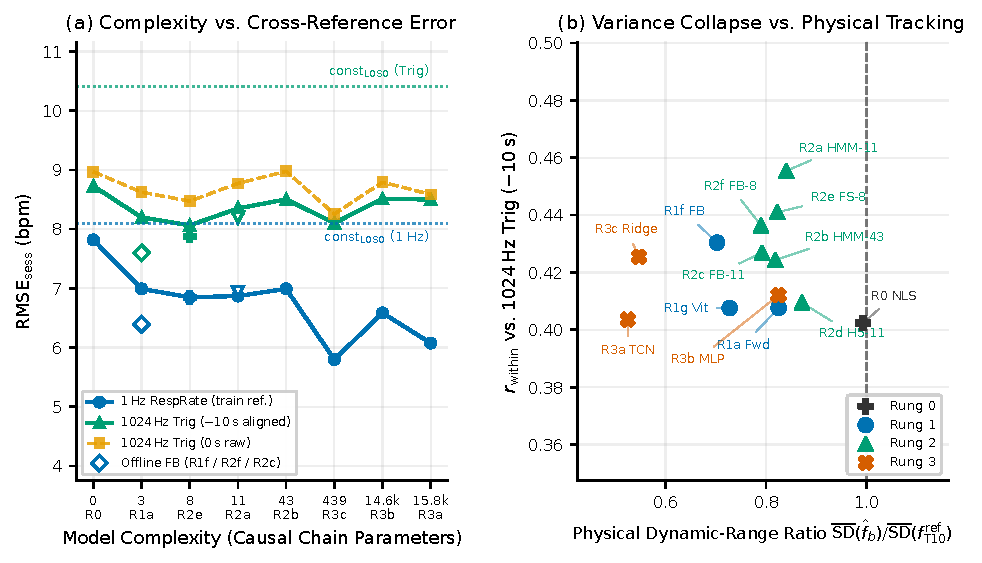
\includegraphics[width=0.94\textwidth]{stage2_complexity_ladder}
  \caption{Four-rung comparison across the training-reference and lag-adjusted trigger
  evaluations. Low one-hertz error from a higher-capacity model does not by itself establish
  transfer to the physical trigger reference.}
  \label{fig:ch4_complexity_ladder}
\end{figure}

\section{Monitor delay, shortcut controls, and physical perturbations}
\label{sec:ch4_controls}

\subsection{Lag profile and the shared trigger correction}
\label{sec:ch4_lag}

In addition to the Stage~2 $[-16,+16]$~s within-session correlation profiles, an independent
post-freeze lag sweep shifts the trigger reference from $-20$ to $+20$~s using the same offset
for each model. Five of the six unshifted models---R0, R1a, R2e, R3c, and R3b---reach their
minimum error or maximum $\rWithin$ at an offset between $+8$ and $+10$~s. For example, R2e
changes from 8.473~bpm at the recorded trigger timing to 8.063~bpm at the project-defined
\texttt{Trig -10 s} alignment, while R1a changes from 8.624 to 8.197~bpm. The common optimum
across architectures is evidence against a model-specific lag search as the explanation for the
observed shift. It is consistent with an effective delay in the monitor reference. The lag
sweep remains observational and cannot separate every source of timing error.

This timing correction is not a learned parameter and is not selected independently for each
held-out infant. It should nevertheless be read as a sensitivity analysis because the trigger and
monitor streams encode different rate definitions, particularly in pause-containing windows.

\subsection{Invariance, causality, gradients, and cache checks}
\label{sec:ch4_implementation_checks}

The structured models were checked against several implementation-level controls. On an
interior rate grid, the Rung~2 operators respond to a rigid $+10$~bpm translation with
numerical error at or below $1.42\times10^{-14}$~bpm for R2e, $7.11\times10^{-15}$~bpm for
R2a, and zero at reported precision for R2b. Under the clinical $[18,90]$~bpm grid
frequency-shift audit ($36\to46$~bpm rigid salience translation), the maximum absolute errors
are $1.20\times10^{-7}$~bpm for R2e, $3.18\times10^{-5}$~bpm for R2a, and
$4.29\times10^{-5}$~bpm for R2b, whereas the absolute-frequency R3c, R3b, and R3a foils show
errors of $3.01$, $5.66$, and $8.86$~bpm. In a separate candidate-grid expansion audit comparing
$[18,90]$ against $[18,120]$~bpm for the flexible-grid Rung~2 decoders, the mean bias shifts
by $0.0000$~bpm for R2e, $0.0188$~bpm for R2a, and $0.0163$~bpm for R2b (the fixed 73-bin
Rung~3 regressors are not defined on the expanded 103-bin grid). On the separate 24~GHz
waveform probe, which changes the input from 36 to 46~bpm, the structured R2e and R2a outputs
change by 9.987 and 10.001~bpm, close to the imposed shift of 10~bpm. The unconstrained R3c,
R3b, and R3a changes are 6.523, 15.043, and 5.465~bpm.

Random future perturbations produce zero reported output difference for the causal forward
decoders and the causal TCN. This is a sequence-level statement about future windows. For
H0-backed models, it does not remove the three-second STFT lookahead described above. The
H5-based R2d ablation removes HPSS/STFT future-frame context, but its block-level normalization
and zero-phase outer bandpass mean that the $0/0$ lookahead entry is not a claim of frame-causal,
zero-latency end-to-end processing. Its one-hertz RMSE is 7.115~bpm, compared with 6.849~bpm for
H0-backed R2e. Because the front end and model both change, this is a bundled comparison, not an
isolated causal effect of STFT lookahead.

Finite-difference checks of the differentiable training gradients found maximum absolute
discrepancies of $4.77\times10^{-9}$ for the tested HMM parameters and
$4.50\times10^{-7}$ for the tested TCN coordinates. The Stage~2 salience extraction was also
recomputed on eight stratified windows from each of 31 session caches: all 248 comparisons
matched the stored features at zero maximum absolute difference for both the H0 and H5 paths.
These audits support implementation fidelity for the tested code and inputs; they do not
validate the model's clinical use.

\subsection{Phase scrambling and synthetic rate sweeps}
\label{sec:ch4_synthetic}

The five-seed phase-scramble control tests whether models continue to follow the reference after
the temporal phase structure of the radar waveform is randomized. For R2e, the one-hertz
$\rmseSess$ rises from 6.849 to $8.361\pm0.105$~bpm, while $\rWithin$ falls from 0.465 to
$-0.006$. The R3 models also show near-zero scrambled within-session correlations. The control
therefore detects dependence on real signal structure in this test, but it is not sufficient to
rule out shortcut learning in the unperturbed recordings.

Synthetic frequency sweeps provide a different test: can the learned mapping follow rates that
were not selected from the NICU cohort's observed distribution? Across stationary 28, 35, 50,
65, and 80~bpm signals and a 30-to-75~bpm chirp (Table~\ref{tab:ch4_synthetic_sweep};
Figure~\ref{fig:ch4_synthetic_sweep}), the passband-safe R2e has low stationary MAE, from 0.01
to 0.04~bpm. The unconstrained R3 errors vary substantially with rate. R3c,
for example, has 7.51~bpm MAE at 28~bpm and 11.18~bpm at 80~bpm; the TCN has 12.45 and
11.14~bpm errors at those rates. These are controlled synthetic signals, so the results
demonstrate behavior under specified mixtures rather than a guarantee for real infants.

\begin{table}[htbp]
  \centering
  \small
  \caption{Zero-touch synthetic frequency sweep. Values are mean absolute error for stationary
  signals and RMSE for the 30-to-75~bpm chirp.}
  \label{tab:ch4_synthetic_sweep}
  \begin{tabular}{@{}lrrrrrr@{}}
    \toprule
    Method & 28~bpm & 35~bpm & 50~bpm & 65~bpm & 80~bpm & Chirp RMSE \\
    \midrule
    R2e FilterSafe-8 & 0.04 & 0.01 & 0.03 & 0.01 & 0.01 & 2.37 \\
    R2a linear HMM & 0.00 & 0.00 & 0.00 & 0.01 & 0.04 & 2.06 \\
    R3c spectral ridge & 7.51 & 5.27 & 2.01 & 3.04 & 11.18 & 2.50 \\
    R3b spectral MLP & 6.64 & 2.88 & 5.43 & 4.81 & 4.28 & 4.15 \\
    R3a causal TCN & 12.45 & 6.06 & 2.80 & 5.81 & 11.14 & 4.99 \\
    \bottomrule
  \end{tabular}
\end{table}

The separate 20~bpm filter-edge diagnostic must not be folded into the 28--80~bpm sweep.
At 20~bpm, the fundamental lies close to the low-frequency skirt of the locked double-pass
Kaiser filter, and the local synthetic test gives 20.00~bpm MAE for R2e and 20.06~bpm for R0.
This exposes a front-end limitation near the passband edge, even though the passband-safe model
performs well over the prespecified 28--80~bpm sweep. The test is not evidence that R2e can
reliably track every rate near the nominal 18~bpm cutoff. It is distinct from the external
20~bpm transfer scenario summarized in Figure~\ref{fig:ch4_rungs} and evaluated in Chapter~6:
that scenario uses a different data source and processing path, so the two results are not
directly interchangeable.

\begin{figure}[htbp]
  \centering
  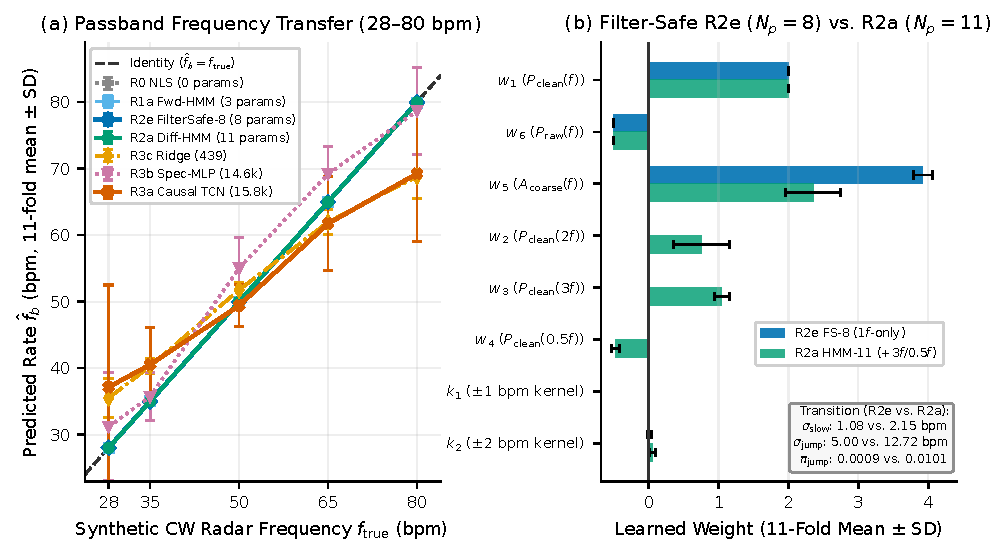
\includegraphics[width=0.94\textwidth]{stage2_synthetic_sweep_and_weights}
  \caption{Passband synthetic rate-sweep results (28--80~bpm) and interpretable Rung~2 weights.
  The frequency sweep reveals rate-dependent errors in unconstrained regressors; the separate
  20~bpm Kaiser low-edge diagnostic is reported in the text.}
  \label{fig:ch4_synthetic_sweep}
\end{figure}

\section{Chapter summary}
\label{sec:ch4_summary}

The Stage~1 gates favor retaining the existing front end: none of the six WP1 I/Q preprocessing
variants shows an adjusted patient-level gain, and the zero-STFT-lookahead HPSS variants do not
establish equivalence to the locked reference. The resulting Rung~1 forward-MMSE filter improves
the one-hertz point estimate without using future sequence windows, while the offline smoothers
show how additional future context can lower error at the cost of latency. The H0-backed causal
decoders still inherit three seconds of STFT lookahead. H5 removes that HPSS/STFT context in its
ablation, but its blockwise normalization and zero-phase filtering also rule out describing the
evaluated path as fully frame-causal and zero-latency.

Across the Stage~2 ladder, the eight-parameter R2e improves on the zero-parameter R0 baseline
with patient-level Holm support against both the one-hertz and lag-adjusted trigger references.
The comparison with the three-parameter R1a filter, however, is Holm-non-significant. Larger
Rung~3 models can rank well against the training reference but show compressed prediction spread,
weaker physical-trigger performance, and poor transfer across synthetic rates. The causal
structured model is therefore a compact, internally supported candidate, not a clinically
validated monitor. The reference delay, pause-dependent target definition, STFT lookahead, and
20~bpm filter-edge behavior remain explicit boundaries. Chapter~5 builds on this model while
examining whether its posterior uncertainty can support selective prediction without hiding
pause-like intervals.
